% METHODS

The LED sample with its metal layers shown in \autoref{fig:metal_layers} was grown by the staff of the course and given to the student group.
To form a working LED from the metal layer sample, the following steps were done at NTNU NanoLab:

\begin{enumerate}
    \item Front contact formation
    \item GaAs contact layer etch
    \item Backside contact formation
    \item Mesa etch, PECVD passivation deposition, and contact annealing
    \item Planarization and passivation layer etch
    \item Pad metallization
\end{enumerate}

\begin{figure}[h]
    \centering
    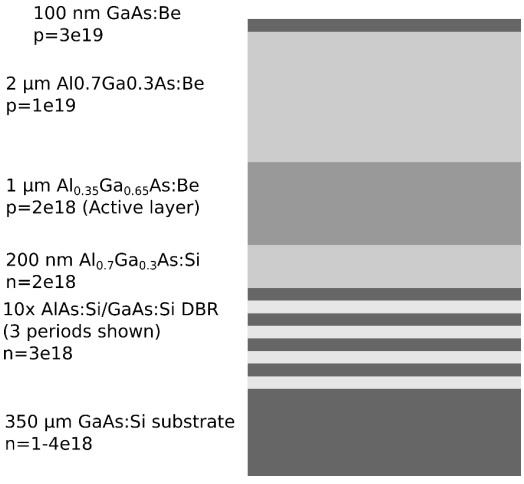
\includegraphics[width=0.45\textwidth]{figures/metal_layers.jpg}
    \caption{
        The metal layers the students got from the course staff to make the LED.
        The layers were grown in the MBE, molecular beam epitaxy, machine at NTNU NanoLab.
        Figure borrowed from the lab manual.
    }
    \label{fig:metal_layers}

\end{figure}

Each step was first done with a GaAs dummy sample to check that the process was working as intended.
After the last step, the LED was ready for testing at a lab at IES, the Department of Electronic Systems at NTNU.


\subsection{LED design}
\label{methods:led_design}

Different finger spacings and finger widths were tested.
An overview schematic of the LED design is shown in \autoref{fig:led_schematic}.
One LED was 1 mm x 1 mm.
The bus bar for contact pad was 1 mm x 300 \textmu m.
The bus bar connecting the fingers was 1 mm x 100 \textmu m.
The fingers were 450 \textmu m long, with widths ranging from 50 \textmu m to 100 \textmu m and spacings ranging from 50 \textmu m to 100 \textmu m.
\textbf{FIX THESE NUMBERS}
\textbf{FIGURE WITH DIFFERENT FINGER WIDTHS AND SPACINGS? CleWin stuff}


\begin{figure}[ht]
    \centering
    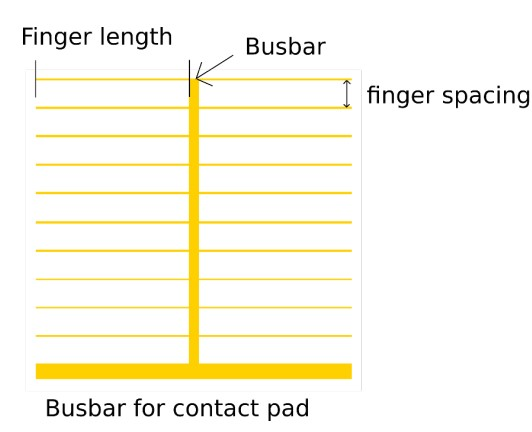
\includegraphics[width=0.45\textwidth]{figures/LED_schematic.jpg}
    \caption{
        Schematic of the LED design.
        Figure borrowed from the lab manual.
    }
    \label{fig:led_schematic}
\end{figure}


\subsection{Front contact formation}
\label{methods:front_contact}

The bus bar and its fingers were formed with lithography and lift-off.
A dose test was done to find the optimal dose and developing time for the resist, ensuring an undercut.
An image of the achieved undercut in the dose test is shown in a SEM image in \autoref{results} in \autoref{fig:undercut}.
The optimal dose was 1300 mJ/cm$^2$ and the optimal developing time was 5 min.
All temperatures are probably some degrees off, since the hot plates at NanoLab havt not been calibrated for many years.
\textbf{FIX THESE NUMBERS}
Negative photoresist was used, and the steps were done in the following order:
\begin{enumerate}
    \item Cleaned the sample with acetone and IPA.
    \item Dehydration baked at 110 \textdegree C for 4 min. ???
    \item Spin coated MAN 440 resist at 4000 rpm for 30 s with 1000 rpm/s acceleration.
    \item Cleaned the backside.
    \item Soft baked at 95 \textdegree C for 5 min.
    \item Exposed the pattern at 1300 mJ/cm$^2$ in the MLA.
    \item Developed in maD-332S developer for 5 min.
    \item Optical inspected the pattern.
    \item Teaching assistants metallized the pattern with Au. \textbf{Au or Pd/Ti/Pt/Au?}
    \item Lift-off with acetone.
\end{enumerate}

Unfortunately, the students mixed up the developer with another group the first time, and had to start over.
The optical inspection before round number two showed some bubbles on the wafer, which was probably caused by the wrong developer.
The wafer was cleaned thuroghly with acetone and IPA before the second round, but some residue might have been left behind.

Another problem was that the dose test were done with a resist that got emtied, and the students had to use a new resist for the actual process.
The new resist needed some more time in developer, which gave an undercut but damaged the alignment marks and the thinnest fingers.
\textbf{Was this the new resist with a weird dev time?}




\subsection{GaAs contact layer etch}
\label{methods:wet_etch}
The heavy p-doped GaAs layer at the top of the metal stack was etched away to allow light to pass through the LED.
The deposited Au fingers were measured to be 250 nm high in the profilometer.
Measuring the Au height was important for the later measurement of the etch debth of the 100 nm GaAs layer.
The Au fingers were protected with a positive photoresist before the wet etch.
Optimal dose for the positive photoresist was found to be 130 mJ/cm$^2$. \textbf{True?}
The preperation was done with the following steps:
\begin{enumerate}
    \item Cleaned the sample with IPA.
    \item Dehydration baked at 110 \textdegree C for 4 min. ??
    \item Spin coated SPR 700 resist at 4000 rpm for 34 s with 1000 rpm/s acceleration.
    \item Soft baked at 95 \textdegree C for 1 min.
    \item Aligned the pattern in the MLA. The alignment marks were badly damaged, so the alignment was not perfect. See \autoref{fig:alignment}.
    \item Exposed the pattern at 130 mJ/cm$^2$ in the MLA.
    \item Post exposure baked at 115 \textdegree C for 1 min.
    \item Developed in maD-332S developer for 30 sec.
    \item Optical inspected the pattern to see if it covered the Au fingers.
\end{enumerate}

The students tried to use the Verniers to calculate the misalignment, but the Verniers were too badly damaged to get a number.
The wet etch was done at the chemial clanroom at NTNU NanoLab, with NH4OH:H2O2:H20 in 3:1:300 ratio.
The etch debth was tested on the GaAs dummy sample, and measured with the profilometer to figure out a etch time which would remove 100 nm of GaAs.
The GaAs dummy was etched 50 nm at the first run, thus the time was doubled for the LED etch to achieve 100 nm.
The etch steps were as follows:

\begin{enumerate}
    \item All equipment and chemicals were placed in the avtrekksskap. ??????
    \item 3 mL NH$_3$ was added to the etch tank with 300 ml H$_2$O.
    \item 1 mL H$_2$O$_2$ was added to the etch tank.
    \item The sample was placed in the etch tank for 60 sec. \textbf{True time?}
    \item The sample was rinsed with H$_2$O and cleaned on the backside.
    \item The protective photoresist was removed with acetone and IPA before profilometer measurement.
    \item The etch debth was measured with the profilometer.
\end{enumerate}



\subsection{Backside contact formation (step 3 or 4?)}
\label{methods:backside_metallization}
The backside of the LED wafer sample was metallized with Au to form the backside contact.
The metallization was done by the teaching assistants, but the students had to protect the frontside with a photoresist.
The student selected the positive photoresist SPR 700, since that one gave better results than MAN 440.
\textbf{This is true? SPR 700 for protection?}
The frontside protection was done with the following steps:
\begin{enumerate}
    \item Cleaned the sample with acetone and IPA.
    \item Dehydration baked at 110 \textdegree C for 4 min. ??
    \item Spin coated SPR 700 resist at 4000 rpm for 34 s with 1000 rpm/s acceleration.
    \item Soft baked at 95 \textdegree C for 1 min.
    \item No exposure was done, since the whole frontside needed to be protected.
    \item Post exposure baked at 115 \textdegree C for 1 min.
    \item Developed in maD-332S developer for 30 sec.
    \item Optically inspected the pattern to see if it covered the whole frontside.
\end{enumerate}


\subsection{Mesa etch, PECVD passivation deposition, and contact annealing}
\label{methods:PECVD}
In one session the students did the mesa etch, passivation deposition and contact annealing.
The mesa etch was done with a wet etch with H3PO4:H2O2:H2O 5:5:15, with the goal of seperating the 16 LEDs.
The mesa etch had to get through the two p-doped Al$_0.7$Ga$_0.3$As layers, i.e. had to be deeper than 3 \textmu m.
The preperation for the mesa etch was to add a positive photoresist mesa mask, which was done in the following steps:

\begin{enumerate}
    \item Cleaned the sample with acetone and IPA.
    \item Dehydration baked at 110 \textdegree C for 4 min. ??
    \item Spin coated SPR 700 resist at 4000 rpm for 34 s with 1000 rpm/s acceleration.
    \item Soft baked at 95 \textdegree C for 1 min.
    \item Aligned the pattern in the MLA.
    \item Exposed the pattern at 130 mJ/cm$^2$ in the MLA.
    \item Post exposure baked at 115 \textdegree C for 1 min.
    \item Developed in maD-332S developer for 30 sec.
    \item Optically inspected the pattern to see if it covered the LEDs.
\end{enumerate}

The mesa etch and passivation deposition was done in parallell at NTNU NanoLab.
The wet etch was first done on the GaAs dummy to test the etch time, and the students figured out that 1 min 45 sec would be sufficient to etch through the two p-doped layers.
The optimal thickness for the passivation layer was 253 nm to minimize reflection.
The following steps were done:

\begin{enumerate}
    \item Deposited Si$_3$N$_4$ passivation layer on Si to find an optimal layer thickness. The recipe used was "(OPT) Si3N4" for 10 min.
    \item Wet etch of the dummy to find a suitable etch time. This etch time was 1 min 30 sec, which was increased by 15 sec for the LED etch.
    \item The wet etch was done with H3PO4:H2O2:H2O 5:5:15 mL.
    \item The resist was stripped of the dummy, and the etch debth was measured with the profilometer.
    \item The inferometer was used to measure the passivation layer deposition thickness.
    \item The LED was mesa wet etched as the dummy was, but with 1 min 45 sec etch time.
    \item The etch debth was controlled to be deeper than 3 \textmu m in the profilometer.
    \item PECVD passivation layer deposition was done on the LED and the dummy with the same recipe as the Si test, because the recipe was found to be good enough. \textbf{True?}
    \item The last step was the contact annealing, which was done at 400 \textdegree C for 30 sec in the RTP.
\end{enumerate}



% \subsection{Passivation deposition and contact annealing}
% \label{methods:passivation}



\subsection{Planarization and passivation layer etch}
\label{methods:Planarization}

The planarization was done by the students, which the passivation layer etch was done by the teaching assistants.
The planarization and preperation for the passivation layer etch was to add a thick positive photoresist with a mask opening on the bottom bus bar, and was done in the following steps:

\begin{enumerate}
    \item Cleaned the sample with acetone and IPA.
    \item Dehydration baked at 110 \textdegree C for 4 min. ??
    \item Spin coated AZ5214E positive resist at 1000 rpm for 34 sec with 250 rpm/s acceleration.
    \item Soft baked at 95 \textdegree C for 1 min.
    \item Exposed the pattern at 80 mJ/cm$^2$ in the MLA.
    \item Developed in 70:30 ma-D 332S:H2O developer for 1 min 30 sec.
    \item Hard baked at 175 \textdegree C for 15 min.
    \item Optical inspection of the pattern.
    \item Teaching assistants preformed HF etch to expose the Au in the bottom bus bar.
\end{enumerate}



\subsection{Pad metallization}
\label{methods:pad_metallization}

The students did the preperation for the pad metallization, while the teaching assistants did the pad metallization.
The lab manual said to use negative photoresist, but the students used positive photoresist, since that gave better results and does actually work for lift-off. % nevn i diskusjon ??
The preperation was to make a positive photoresist mask for the pad metallization, and was done in the following steps:
\begin{enumerate}
    \item Cleaned the sample with IPA.
    \item Dehydration baked at 110 \textdegree C for 4 min. ??
    \item Spin coated SPR 700 resist at 4000 rpm for 34 s with 1000 rpm/s acceleration.
    \item Soft baked at 95 \textdegree C for 1 min.
    \item Exposed the pattern at 80 mJ/cm$^2$ in the MLA.
    \item Post exposure baked at 115 \textdegree C for 1 min.
    \item Developed in maD-332S developer for 30 sec.
    \item Optical inspected the pattern to see if it covered the bottom bus bar and an area below.
    \item Handed in the sample to the teaching assistants, who did the pad metallization with Au.
    \item The students did the lift-off of the resist with acetone.
\end{enumerate}


\subsection{LED testing/characterization}
\label{methods:LED_testing}
After all these steps the LED was ready for testing.
Testing was done at IES, with \dots

